\section{Desarrollo}

\subsection{Algoritmo de Kruskal}

\begin{figure}[H]
\centering

\begin{subfigure}{0.3\textwidth}
\centering

\includegraphics[width=\linewidth]{rsc/img/k1.png}
\end{subfigure}
\begin{subfigure}{0.3\textwidth}
\centering

\includegraphics[width=\linewidth]{rsc/img/k2.png}
\end{subfigure}
\begin{subfigure}{0.3\textwidth}
\centering

\includegraphics[width=\linewidth]{rsc/img/k3.png}
\end{subfigure}

\vspace{0.3cm}

\begin{subfigure}{0.3\textwidth}
\centering

\includegraphics[width=\linewidth]{rsc/img/k4.png}
\end{subfigure}
\begin{subfigure}{0.3\textwidth}
\centering

\includegraphics[width=\linewidth]{rsc/img/k5.png}
\end{subfigure}
\begin{subfigure}{0.3\textwidth}
\centering

\includegraphics[width=\linewidth]{rsc/img/k6.png}
\end{subfigure}

\vspace{0.3cm}

\begin{subfigure}{0.3\textwidth}
\centering
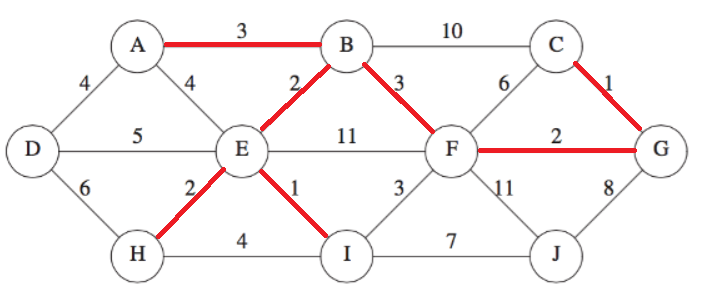
\includegraphics[width=\linewidth]{rsc/img/k7.png}
\end{subfigure}
\begin{subfigure}{0.3\textwidth}
\centering
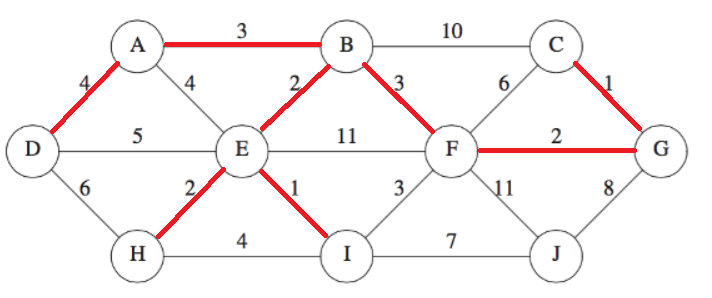
\includegraphics[width=\linewidth]{rsc/img/k8.png}
\end{subfigure}
\begin{subfigure}{0.3\textwidth}
\centering
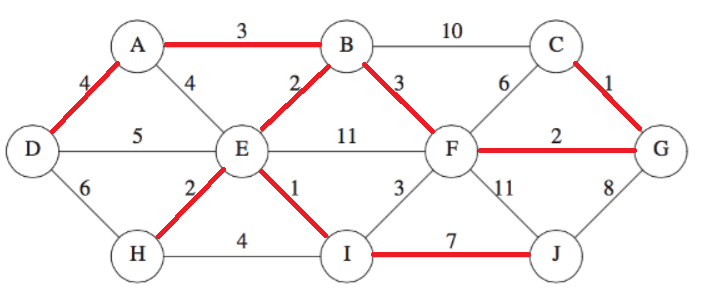
\includegraphics[width=\linewidth]{rsc/img/k9.png}
\end{subfigure}

\caption{Procedimiento del algoritmo de Kruskal}\label{fig:kruskal}
\end{figure}

Ruta seguida por el algoritmo de Kruskal:
\begin{table}[H]
    \centering
    \begin{tabular}{|c|c|}
        \hline
        Vértice & Grado \\
        \hline
        (E,I) & 1 \\
        (C,G) & 1 \\
        (E,H) & 2 \\
        (E,B) & 2 \\
        (F,G) & 2 \\
        (B,F) & 3 \\
        (F,I) & X \\
        (B,A) & 3 \\
        (D,A) & 4 \\
        (A,E) & X \\
        (H,I) & X \\
        (D,E) & X \\
        (D,H) & X \\
        (F,C) & X \\
        (I,J) & 7 \\
        \hline
        Total & 25 \\
        \hline
    \end{tabular}
    \caption{Costo total Algoritmo de Kruskal}\label{tab:grados_vertices}
\end{table}

%%%%%%%%%%%%%%%%%%%%%%%%%%%%%%%%%%%%%%%%%%%%%%%%%%%%%%%%%%%%%%%%%%%%%
\subsection{Algoritmo de Prim}

\begin{figure}[H]
\centering

\begin{subfigure}{0.3\textwidth}
\centering
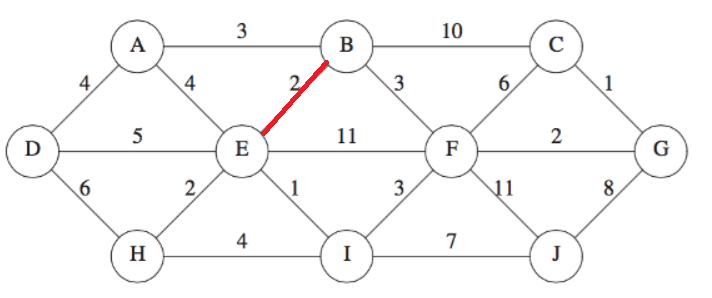
\includegraphics[width=\linewidth]{rsc/img/p1.png}
\end{subfigure}
\begin{subfigure}{0.3\textwidth}
\centering
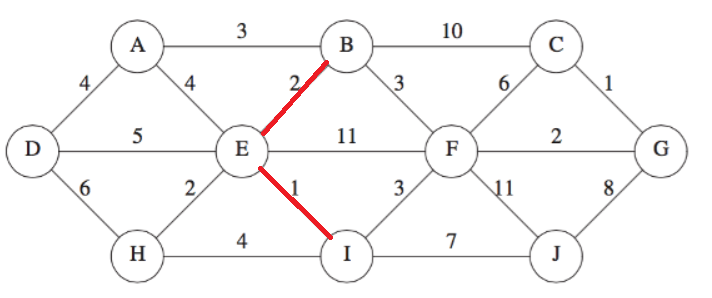
\includegraphics[width=\linewidth]{rsc/img/p2.png}
\end{subfigure}
\begin{subfigure}{0.3\textwidth}
\centering
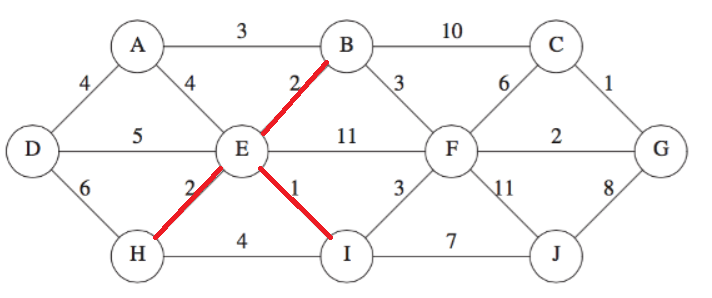
\includegraphics[width=\linewidth]{rsc/img/p3.png}
\end{subfigure}

\vspace{0.3cm}

\begin{subfigure}{0.3\textwidth}
\centering
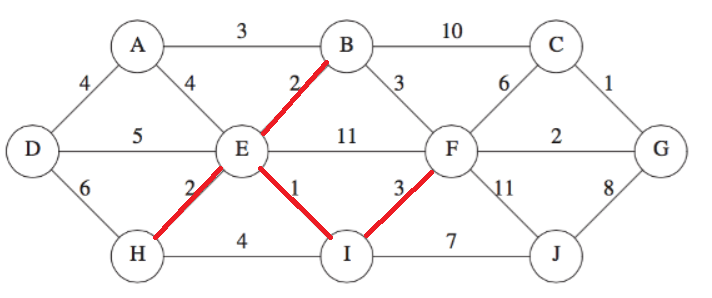
\includegraphics[width=\linewidth]{rsc/img/p4.png}
\end{subfigure}
\begin{subfigure}{0.3\textwidth}
\centering
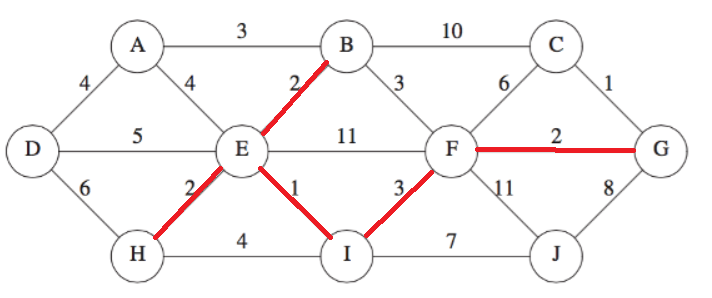
\includegraphics[width=\linewidth]{rsc/img/p5.png}
\end{subfigure}
\begin{subfigure}{0.3\textwidth}
\centering
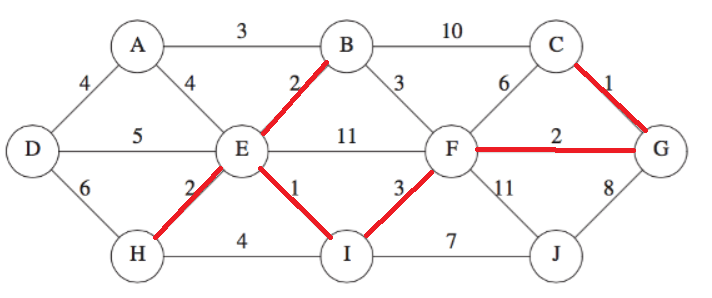
\includegraphics[width=\linewidth]{rsc/img/p6.png}
\end{subfigure}

\vspace{0.3cm}

\begin{subfigure}{0.3\textwidth}
\centering
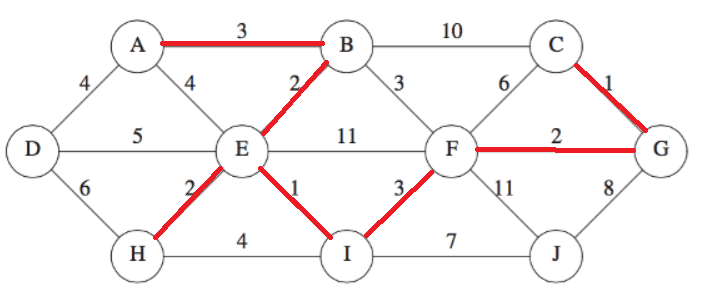
\includegraphics[width=\linewidth]{rsc/img/p7.png}
\end{subfigure}
\begin{subfigure}{0.3\textwidth}
\centering
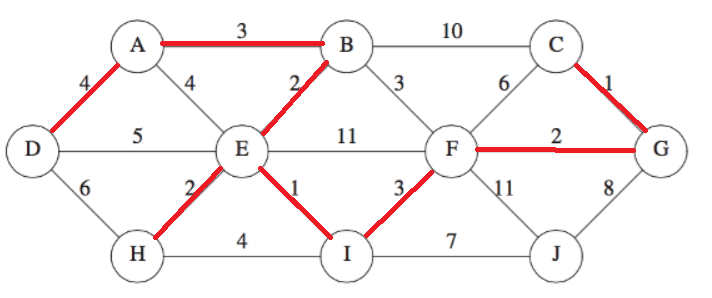
\includegraphics[width=\linewidth]{rsc/img/p8.png}
\end{subfigure}
\begin{subfigure}{0.3\textwidth}
\centering
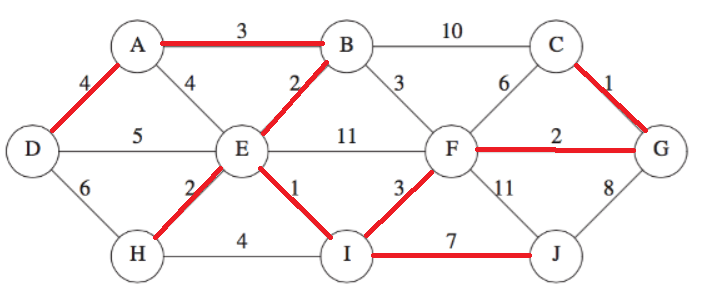
\includegraphics[width=\linewidth]{rsc/img/p9.png}
\end{subfigure}

\caption{Procedimiento del algoritmo de Prim}\label{fig:prim}
\end{figure}

Ruta seguida por el algoritmo de Prim:
\begin{table}[H]
    \centering
    \begin{tabular}{|c|c|}
        \hline
        Vértice & Grado \\
        \hline
        (B,E) & 2 \\
        (E,I) & 1 \\
        (E,H) & 2 \\
        (I,F) & 3 \\
        (F,G) & 2 \\
        (G,C) & 1 \\
        (B,A) & 3 \\
        (A,D) & 4 \\
        (I,J) & 7 \\
        \hline
        Total & 25 \\
        \hline
    \end{tabular}
    \caption{Costo total Algoritmo de Prim}\label{tab:grados_vertices}
\end{table}

%%%%%%%%%%%%%%%%%%%%%%%%%%%%%%%%%%%%%%%%%%%%%%%%%%%%%%%%%%%%%%%%%%%%%
\subsection{Algoritmo de Sollin}

\begin{figure}[H]
\centering

\begin{subfigure}{0.45\textwidth}
\centering
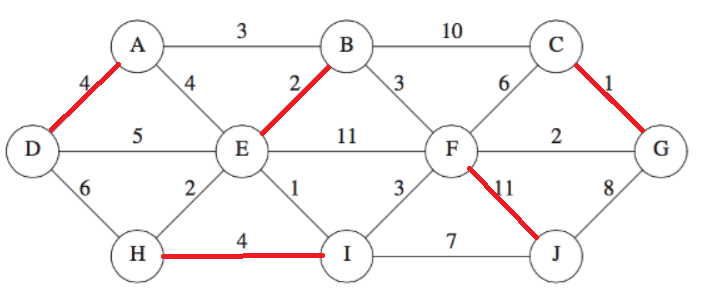
\includegraphics[width=\linewidth]{rsc/img/s1.png}
\end{subfigure}
\begin{subfigure}{0.45\textwidth}
\centering
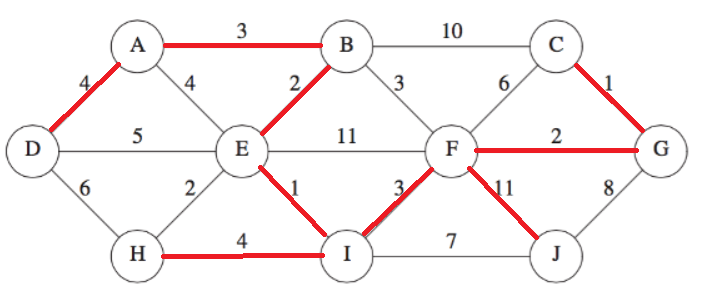
\includegraphics[width=\linewidth]{rsc/img/s2.png}
\end{subfigure}

\caption{Procedimiento del algoritmo de Sollin}\label{fig:sollin}
\end{figure}

Ruta seguida por el algoritmo de Sollin:
\begin{table}[H]
    \centering
    \begin{tabular}{|c|c|c|}
        \hline
        Vértice & Grado & Paso \\
        \hline
        (B,E) & 2 & \\
        (C,G) & 1 & \\
        (A,D) & 4 & 1\\
        (H,I) & 4 & \\
        (F,J) & 11 & \\
        \hline
        (A,B) & 3 & \\
        (E,I) & 1 & 2\\
        (F,G) & 2 & \\
        (E,F) & 3 & \\
        \hline
        Total & 31 & \\
        \hline
    \end{tabular}
    \caption{Costo total Algoritmo de Sollin}\label{tab:grados_vertices}
\end{table}

\subsection{Resultados}

\subsubsection{Kruskal}
\begin{figure}[H]
    \centering
    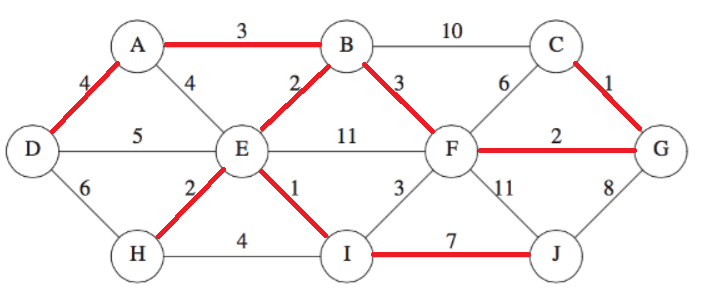
\includegraphics[width=0.75\textwidth]{rsc/img/k9.png}
    \caption{Arbol de Kruskal}\label{fig:Tree_Kruskal}
\end{figure}

\subsubsection{Prim}
\begin{figure}[H]
    \centering
    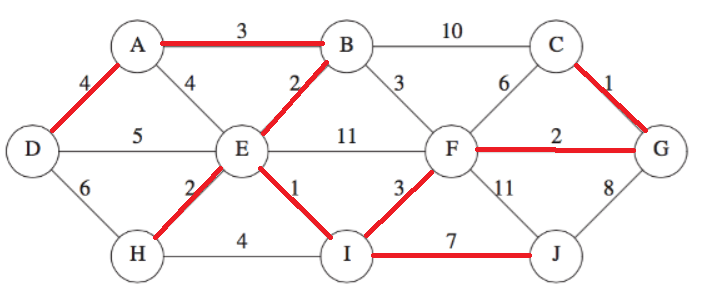
\includegraphics[width=0.75\textwidth]{rsc/img/p9.png}
    \caption{Arbol de Prim}\label{fig:Tree_Prim}
\end{figure}

\subsubsection{Sollin}
\begin{figure}[H]
    \centering
    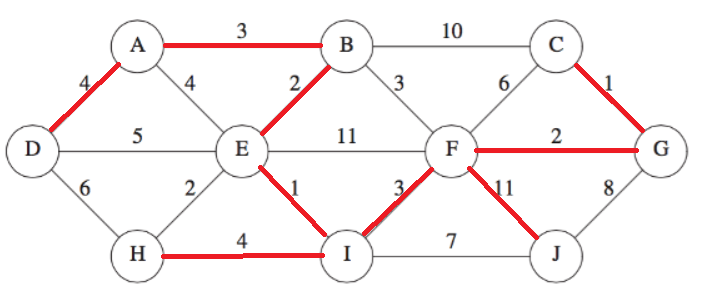
\includegraphics[width=0.75\textwidth]{rsc/img/s2.png}
    \caption{Arbol de Sollin}\label{fig:Tree_Sollin}
\end{figure}